%%%%%%%%%%%%%%%%%%%%%%%%%%%%%%%%%%%%%%%%%%%%%%%%%%%%%%%%%%%%%%%%%%%%%%%%%%%%%%%%%%
\begin{frame}[fragile]\frametitle{}
\begin{center}
{\Large Introduction to Feature-based Design}
\end{center}
\end{frame}

%%%%%%%%%%%%%%%%%%%%%%%%%%%%%%%%%%%%%%%%%%%%%%%%%%%%%%%%%%%%%%%%%%%%%%%%%%%%%%%%%%
\begin{frame}[fragile]\frametitle{Feature-Based Solid Modeling}

\begin{itemize}
\item Parts modeled by adding features to a base part
\item Features represent ``operations'': holes, ribs, fillets, chamfers, slots, pockets, etc.
\item Material can be added or subtracted
\item Features can be created by extrusion, sweeping, revolving, etc.
\end{itemize}

\end{frame}

%%%%%%%%%%%%%%%%%%%%%%%%%%%%%%%%%%%%%%%%%%%%%%%%%%%%%%%%%%%%%%%%%%%%%%%%%%%%%%%%%%
\begin{frame}[fragile]\frametitle{Feature-based Modeling Process}

\begin{itemize}
\item Create base part
\item Add features until final shape is achieved
\end{itemize}

			\begin{center}
	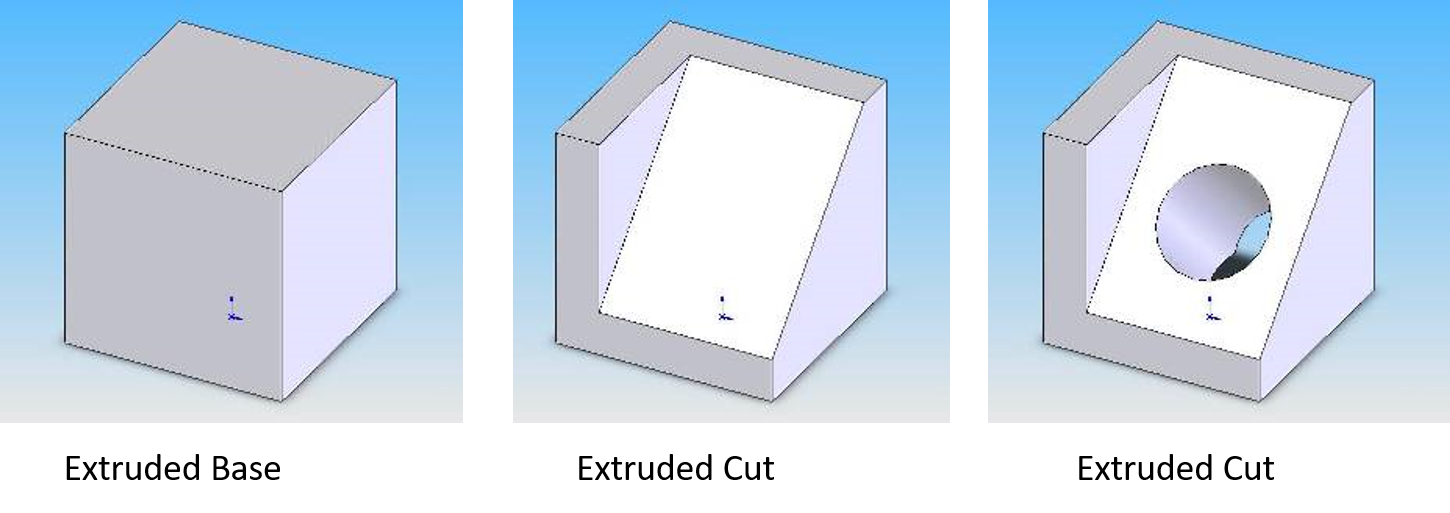
\includegraphics[width=0.6\linewidth,keepaspectratio]{geomod21}
			\end{center}
\end{frame}

%%%%%%%%%%%%%%%%%%%%%%%%%%%%%%%%%%%%%%%%%%%%%%%%%%%%%%%%%%%%%%%%%%%%%%%%%%%%%%%%%%
\begin{frame}[fragile]\frametitle{Feature History Trees}

\begin{itemize}
\item Most feature-based modelers show the features and their order in a graphical tree view
\item This view has different names, depending on the software
\end{itemize}
\end{frame}

%%%%%%%%%%%%%%%%%%%%%%%%%%%%%%%%%%%%%%%%%%%%%%%%%%%%%%%%%%%%%%%%%%%%%%%%%%%%%%%%%%
\begin{frame}[fragile]\frametitle{Feature-based Modeling Software}

			\begin{center}
	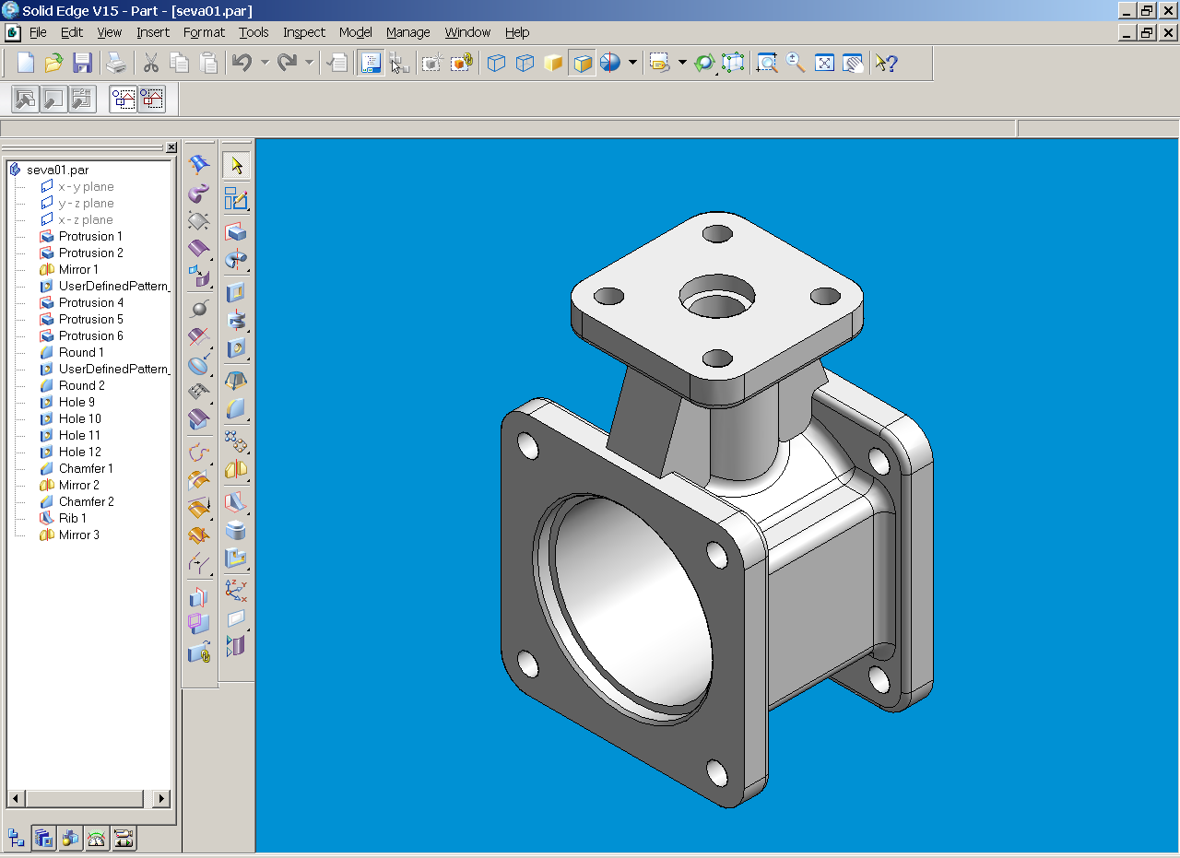
\includegraphics[width=0.8\linewidth,keepaspectratio]{geomod22}
			\end{center}
\end{frame}

%%%%%%%%%%%%%%%%%%%%%%%%%%%%%%%%%%%%%%%%%%%%%%%%%%%%%%%%%%%%%%%%%%%%%%%%%%%%%%%%%%
\begin{frame}[fragile]\frametitle{Feature-based Modeling Software}

			\begin{center}
	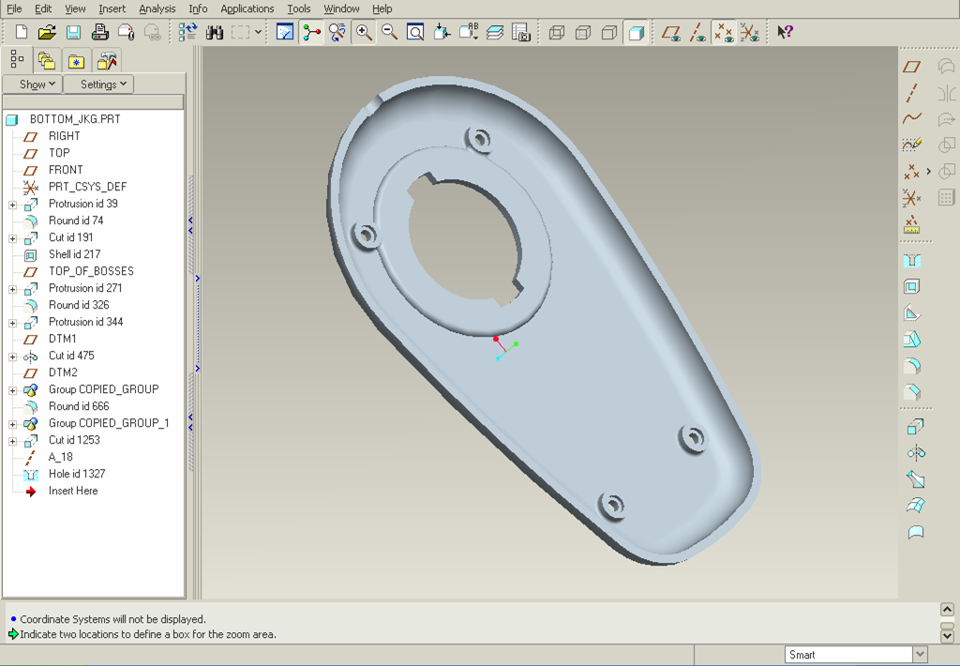
\includegraphics[width=0.8\linewidth,keepaspectratio]{geomod23}
			\end{center}
\end{frame}

%%%%%%%%%%%%%%%%%%%%%%%%%%%%%%%%%%%%%%%%%%%%%%%%%%%%%%%%%%%%%%%%%%%%%%%%%%%%%%%%%%
\begin{frame}[fragile]\frametitle{Feature-based Modeling Software}

			\begin{center}
	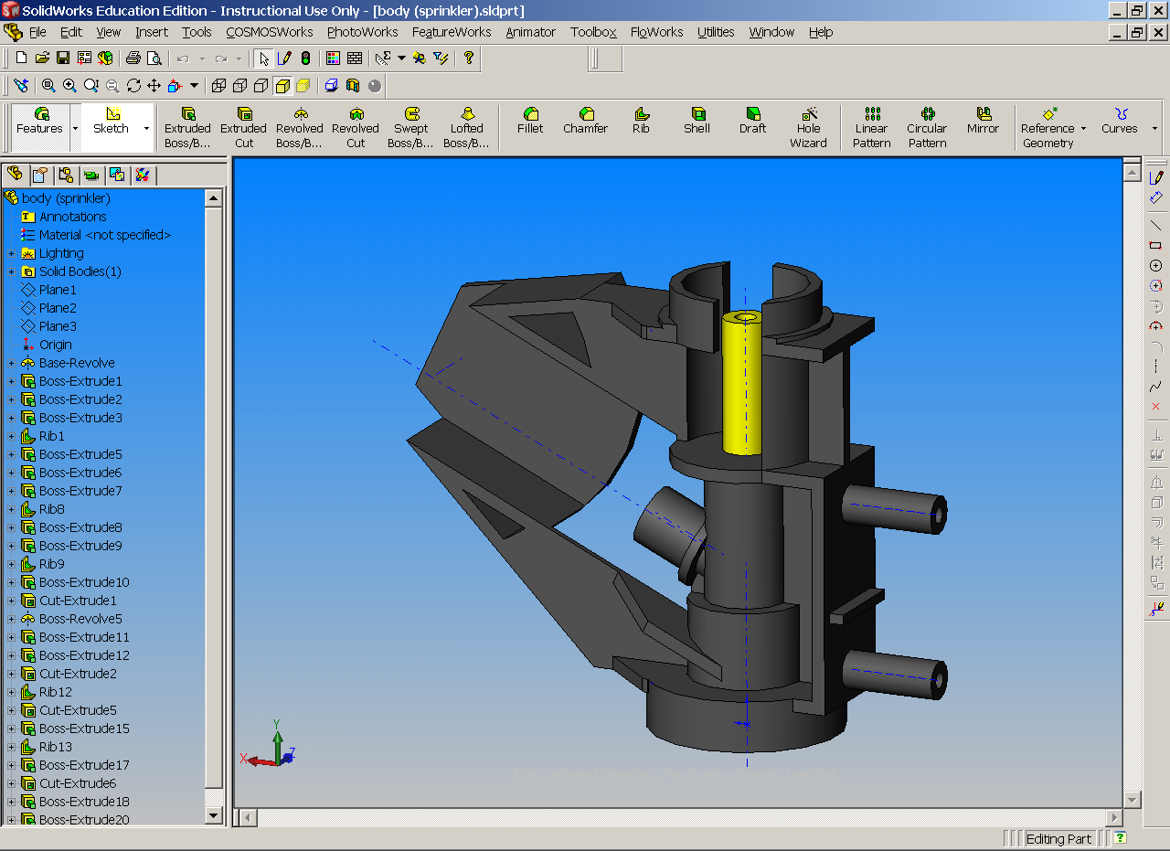
\includegraphics[width=0.8\linewidth,keepaspectratio]{geomod24}
			\end{center}
\end{frame}

%%%%%%%%%%%%%%%%%%%%%%%%%%%%%%%%%%%%%%%%%%%%%%%%%%%%%%%%%%%%%%%%%%%%%%%%%%%%%%%%%%
\begin{frame}[fragile]\frametitle{}
\begin{center}
{\Large FBD: Power of Editing }
\end{center}
\end{frame}

%%%%%%%%%%%%%%%%%%%%%%%%%%%%%%%%%%%%%%%%%%%%%%%%%%%%%%%%%%%%%%%%%%%%%%%%%%%%%%%%%%
\begin{frame}[fragile]\frametitle{Modifying Parts}

\begin{itemize}
\item The part is created from the history tree
\item Features can be added, deleted and re-ordered
\item Feature parameters can be changed
\end{itemize}
\end{frame}


%%%%%%%%%%%%%%%%%%%%%%%%%%%%%%%%%%%%%%%%%%%%%%%%%%%%%%%%%%%%%%%%%%%%%%%%%%%%%%%%%%
\begin{frame}[fragile]\frametitle{Editing Work-flow}

		Hole is to be changed.
		
			\begin{center}
	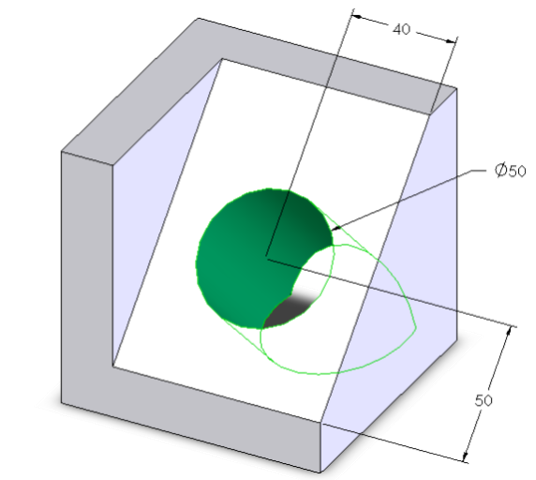
\includegraphics[width=0.6\linewidth,keepaspectratio]{geomod25}
			\end{center}
\end{frame}

%%%%%%%%%%%%%%%%%%%%%%%%%%%%%%%%%%%%%%%%%%%%%%%%%%%%%%%%%%%%%%%%%%%%%%%%%%%%%%%%%%
\begin{frame}[fragile]\frametitle{Editing Work-flow}

		Changed radius from $50$ to $20$.Faces-Surfaces outside-inside adjust.
		
		
			\begin{center}
	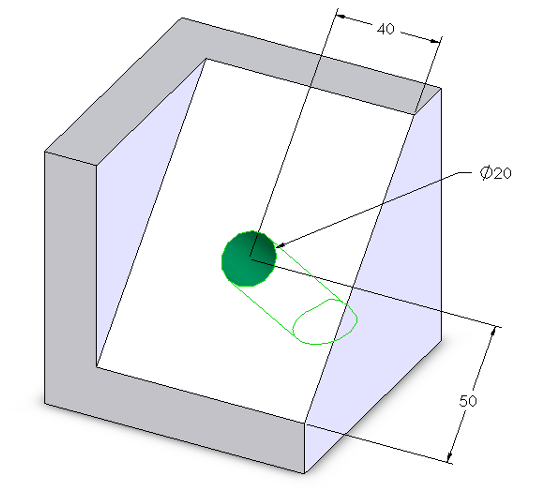
\includegraphics[width=0.6\linewidth,keepaspectratio]{geomod26}
			\end{center}
\end{frame}

%%%%%%%%%%%%%%%%%%%%%%%%%%%%%%%%%%%%%%%%%%%%%%%%%%%%%%%%%%%%%%%%%%%%%%%%%%%%%%%%%%
\begin{frame}[fragile]\frametitle{Editing Work-flow}

		Changed location from $40$ to $60$.Faces-Surfaces outside-inside adjust.

			\begin{center}
	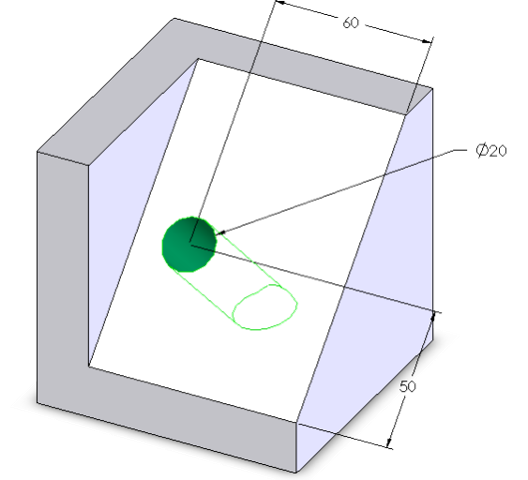
\includegraphics[width=0.6\linewidth,keepaspectratio]{geomod27}
			\end{center}
\end{frame}

%%%%%%%%%%%%%%%%%%%%%%%%%%%%%%%%%%%%%%%%%%%%%%%%%%%%%%%%%%%%%%%%%%%%%%%%%%%%%%%%%%
\begin{frame}[fragile]\frametitle{Design Intent}

\begin{itemize}
\item In parametric modeling, dimensions control the model.
\item Design intent is how your model will react when dimension values are changed. 
\end{itemize}
\end{frame}

%%%%%%%%%%%%%%%%%%%%%%%%%%%%%%%%%%%%%%%%%%%%%%%%%%%%%%%%%%%%%%%%%%%%%%%%%%%%%%%%%%
\begin{frame}[fragile]\frametitle{Design Intent}
 \begin{columns}
  \begin{column}{0.55\linewidth}

\begin{itemize}
\item The drawing shows the intent of the designer that the inclined plane (chamfer) should have a flat area measuring 2.5 inches and that it should start at a point 1.25 inches from the base of the drawing. These parameters are deemed significant.
\item Remember that the placement of dimensions is very important because they are being used to drive the shape of the geometry. will change.
\end{itemize}
  \end{column}%
  \begin{column}{0.45\linewidth}
			\begin{center}
	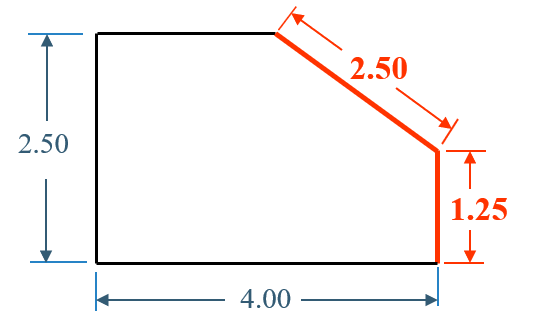
\includegraphics[width=0.9\linewidth,keepaspectratio]{geomod28}
			\end{center}
			
			If the 2.5 in. vertical dimension increases, the 2.5 in. flat across the chamfer will be maintained, but its angle 
  \end{column}
 \end{columns}			
\end{frame}

%%%%%%%%%%%%%%%%%%%%%%%%%%%%%%%%%%%%%%%%%%%%%%%%%%%%%%%%%%%%%%%%%%%%%%%%%%%%%%%%%%
\begin{frame}[fragile]\frametitle{Design Intent}
 \begin{columns}
  \begin{column}{0.55\linewidth}

\begin{itemize}
\item In this drawing, what is important to the designer is the vertical location and horizontal dimension of the chamfer, rather than the flat of the chamfer. 
\item In the last drawing, the designer calls for a specific angle for the chamfer. In this case the angle of the chamfer should be dimensioned.
\end{itemize}
	
  \end{column}%
  \begin{column}{0.45\linewidth}
			\begin{center}
	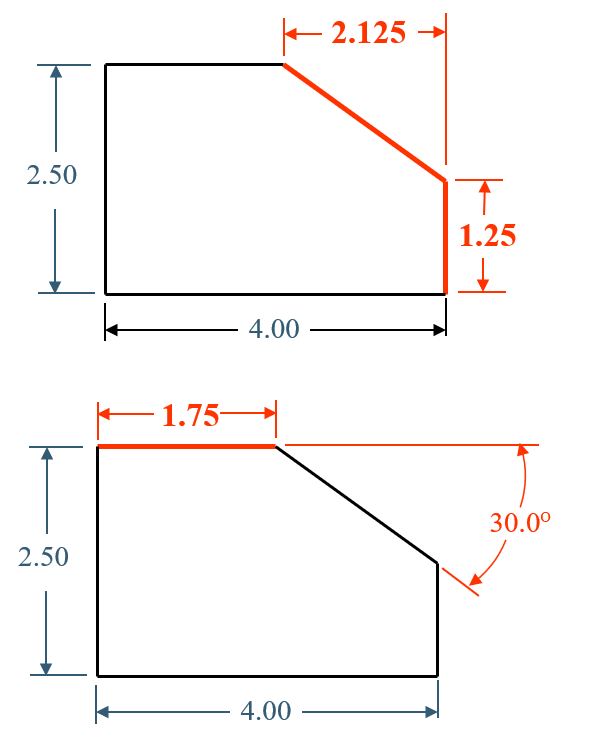
\includegraphics[width=0.9\linewidth,keepaspectratio]{geomod29}
			\end{center}
  \end{column}
 \end{columns}
\end{frame}

%%%%%%%%%%%%%%%%%%%%%%%%%%%%%%%%%%%%%%%%%%%%%%%%%%%%%%%%%%%%%%%%%%%%%%%%%%%%%%%%%%
\begin{frame}[fragile]{Parametric Modeling}
 \begin{columns}
  \begin{column}{0.55\linewidth}

\begin{itemize}
\item The true power of parametric modeling shines through when design changes need to be made. The design modification is made by simply changing a dimension. 
\item Since the counterbore is associated with the top surface of the ring, any changes in the thickness of the ring would automatically be reflected on the counterbore depth.

\end{itemize}
	
  \end{column}%
  \begin{column}{0.45\linewidth}
			\begin{center}
	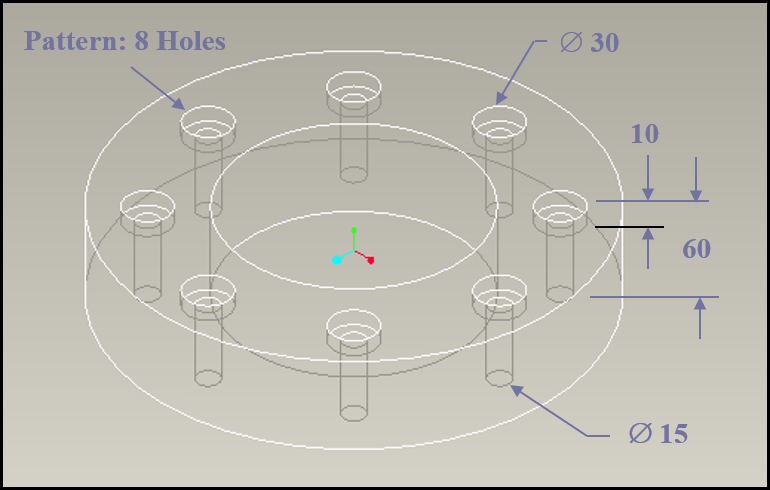
\includegraphics[width=0.9\linewidth,keepaspectratio]{geomod30}
			\end{center}
  \end{column}
 \end{columns}
\end{frame}

%%%%%%%%%%%%%%%%%%%%%%%%%%%%%%%%%%%%%%%%%%%%%%%%%%%%%%%%%%%%%%%%%%%%%%%%%%%%%%%%%%
\begin{frame}[fragile]\frametitle{Sketches}

\begin{itemize}
\item Take the word sketch literally. A sketch should be just that, a sketch.
\item When sketching it is not necessary to create geometry with accuracy. Lines, arcs, and additional geometry need not be created with exact dimensions in mind. 
\item When the dimensions are added, the sketch will change size and shape. This is the essence of Parametric Modeling.
\item In short, the sketch need only be the approximate size and shape of the part being designed. When dimensions are added, they will drive the size and the shape of the geometry.

\end{itemize}
\end{frame}

%%%%%%%%%%%%%%%%%%%%%%%%%%%%%%%%%%%%%%%%%%%%%%%%%%%%%%%%%%%%%%%%%%%%%%%%%%%%%%%%%%
\begin{frame}[fragile]{Features}
 \begin{columns}
  \begin{column}{0.55\linewidth}

Sketched Feature 

\begin{itemize}
\item Create a 2D sketch.
\item Create a feature from the sketch by extruding, revolving, sweeping, lofting and blending.

\end{itemize}
	
  \end{column}%
  \begin{column}{0.45\linewidth}
			\begin{center}
	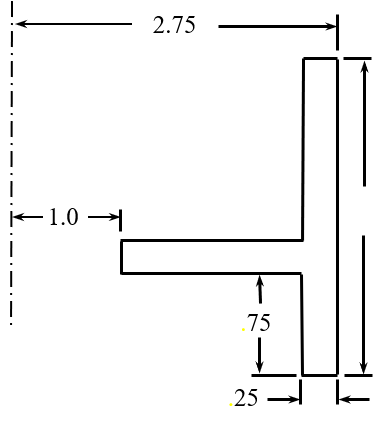
\includegraphics[width=0.5\linewidth,keepaspectratio]{geomod31}
			\end{center}
  \end{column}
 \end{columns}
 
 			\begin{center}
	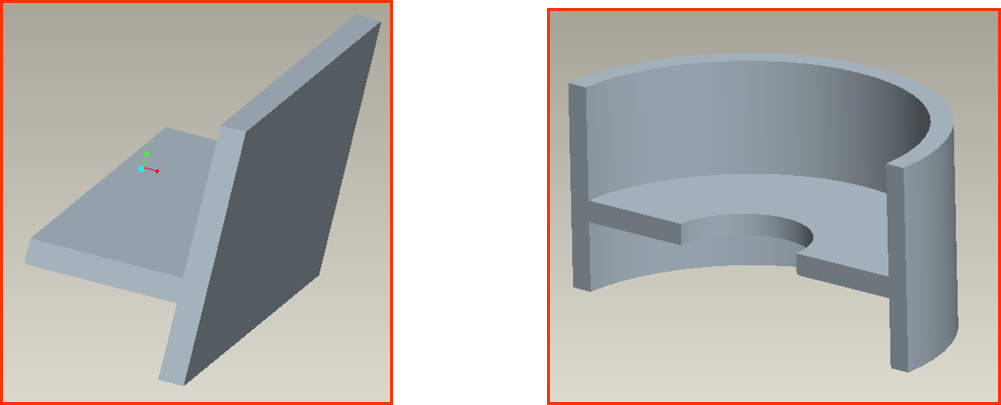
\includegraphics[width=0.6\linewidth,keepaspectratio]{geomod32}
			\end{center}
			
\end{frame}

%%%%%%%%%%%%%%%%%%%%%%%%%%%%%%%%%%%%%%%%%%%%%%%%%%%%%%%%%%%%%%%%%%%%%%%%%%%%%%%%%%
\begin{frame}[fragile]\frametitle{Sweep}

A Sweep feature requires a profile and a path. The profile will follow the path to create the solid.

			\begin{center}
	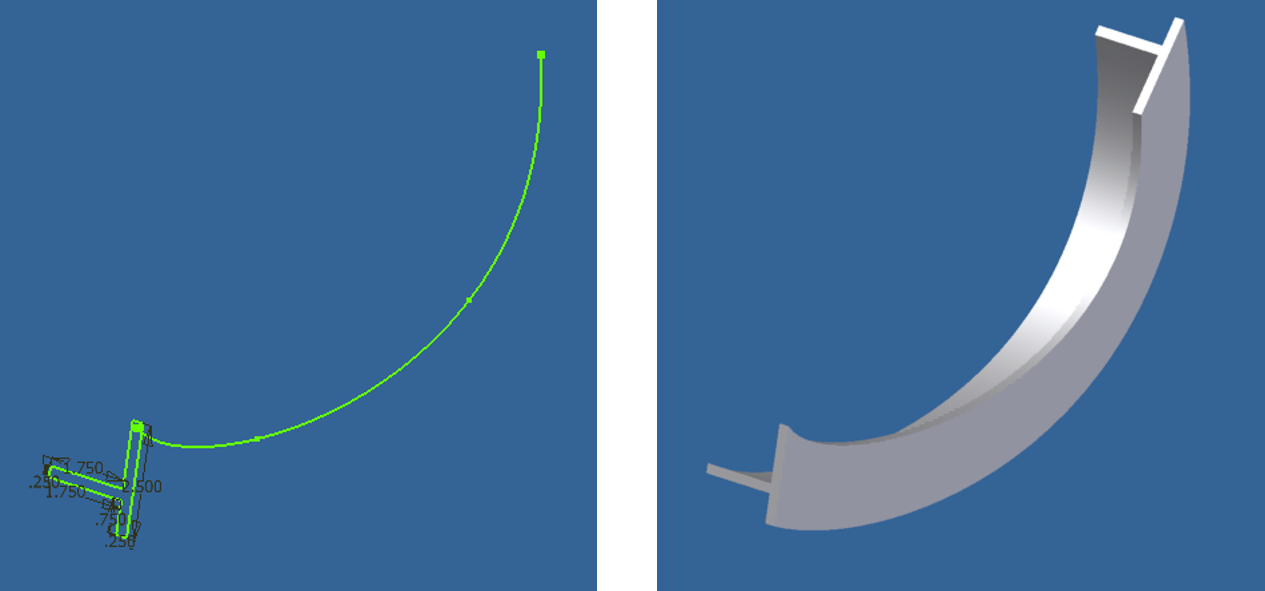
\includegraphics[width=0.9\linewidth,keepaspectratio]{geomod33}
			\end{center}
\end{frame}

%%%%%%%%%%%%%%%%%%%%%%%%%%%%%%%%%%%%%%%%%%%%%%%%%%%%%%%%%%%%%%%%%%%%%%%%%%%%%%%%%%
\begin{frame}[fragile]\frametitle{Loft}

\begin{itemize}
\item Sections (profiles) do not have to be sketched on parallel planes
\item All sections must be either closed or open
\end{itemize}

			\begin{center}
	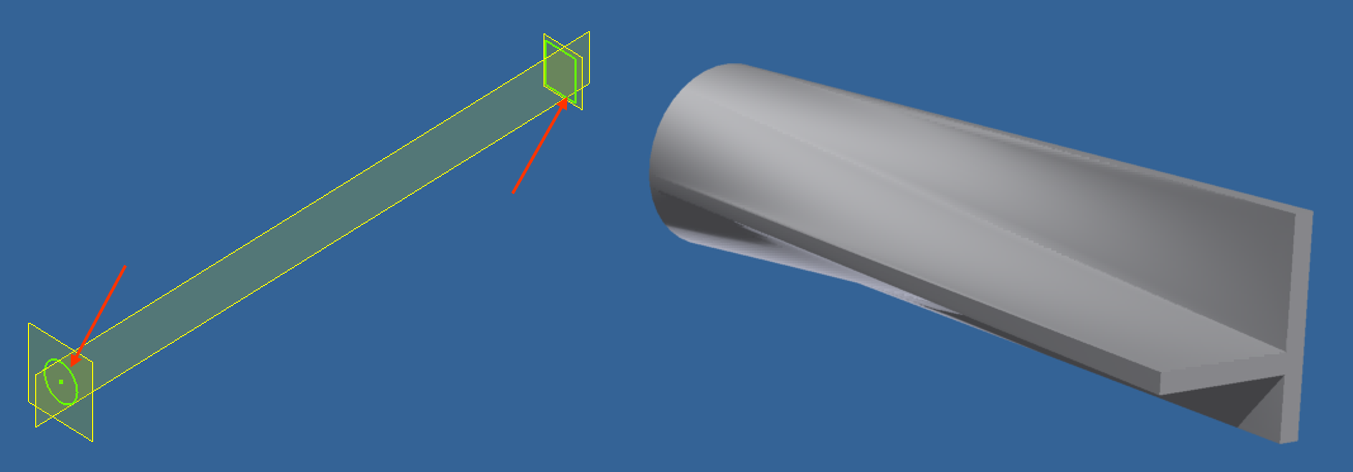
\includegraphics[width=0.9\linewidth,keepaspectratio]{geomod34}
			\end{center}
\end{frame}

%%%%%%%%%%%%%%%%%%%%%%%%%%%%%%%%%%%%%%%%%%%%%%%%%%%%%%%%%%%%%%%%%%%%%%%%%%%%%%%%%%
\begin{frame}[fragile]\frametitle{Creating Features from Sketches}

			\begin{center}
	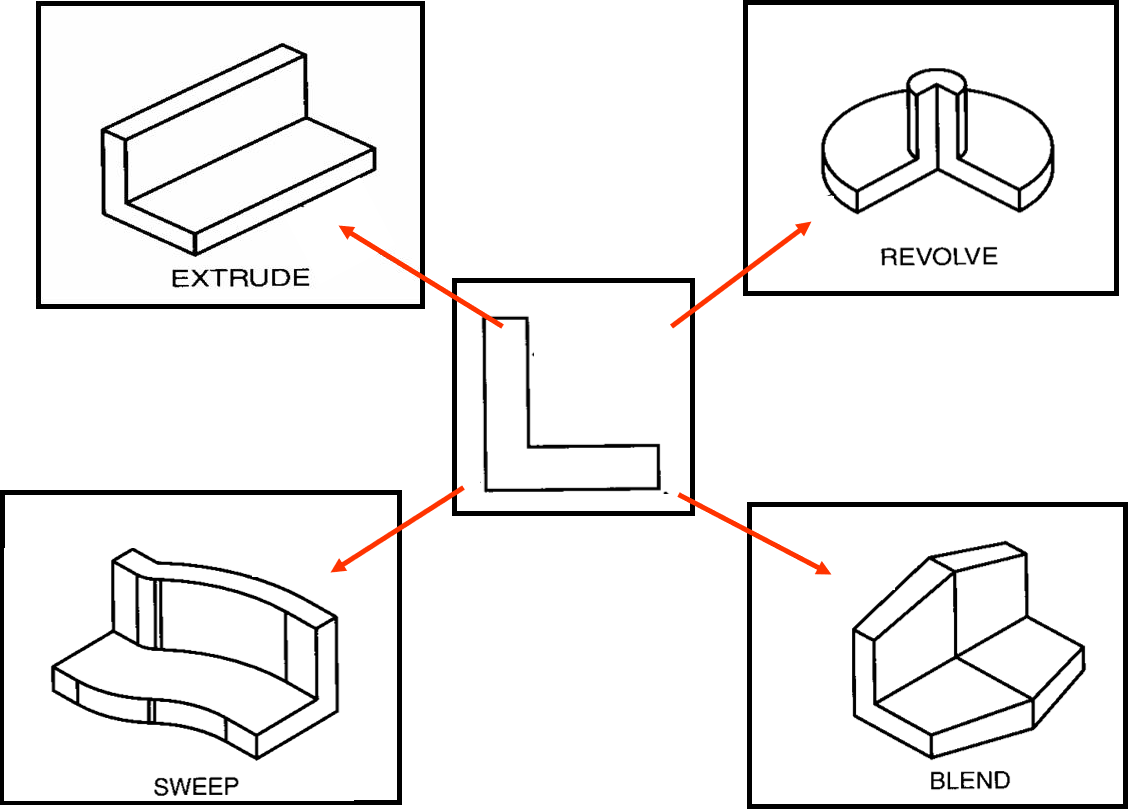
\includegraphics[width=0.9\linewidth,keepaspectratio]{geomod35}
			\end{center}
\end{frame}

%%%%%%%%%%%%%%%%%%%%%%%%%%%%%%%%%%%%%%%%%%%%%%%%%%%%%%%%%%%%%%%%%%%%%%%%%%%%%%%%%%
\begin{frame}[fragile]\frametitle{Tweak Features}

\begin{itemize}
\item Applied feature does not require a sketch.
\item It is applied directly to the model.
\item Fillets and chamfers are very common applied features.
\end{itemize}

			\begin{center}
	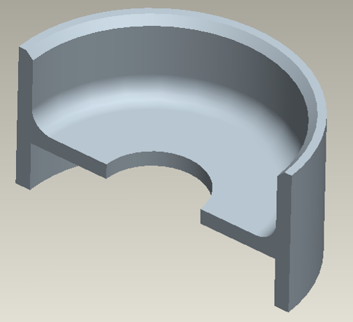
\includegraphics[width=0.9\linewidth,keepaspectratio]{geomod36}
			\end{center}
\end{frame}


%%%%%%%%%%%%%%%%%%%%%%%%%%%%%%%%%%%%%%%%%%%%%%%%%%%%%%%%%%%%%%%%%%%%%%%%%%%%%%%%%%
\begin{frame}[fragile]\frametitle{Shell - Hollow}


			\begin{center}
	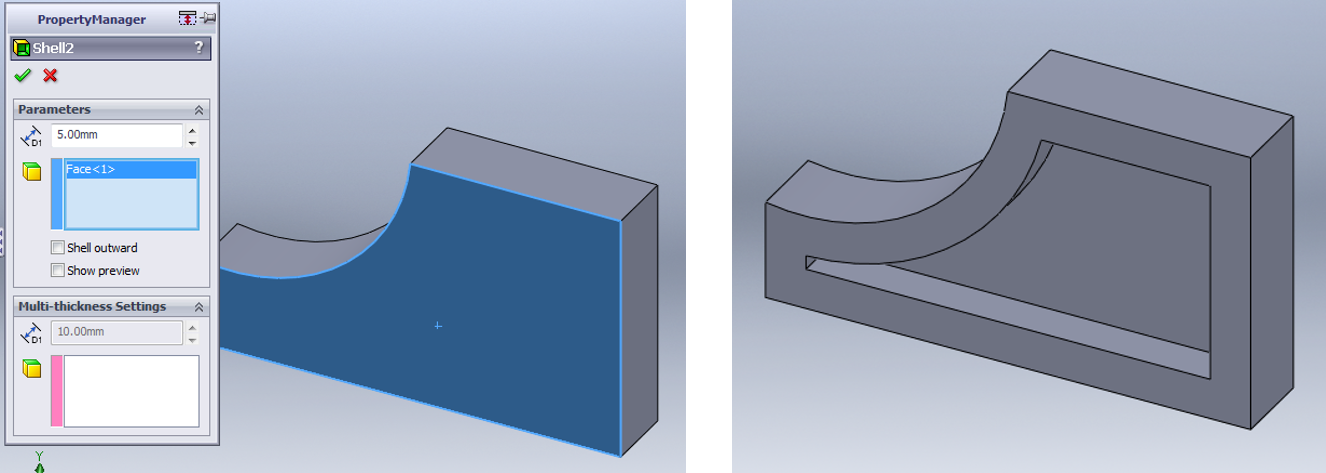
\includegraphics[width=0.9\linewidth,keepaspectratio]{geomod37}
			\end{center}
\end{frame}

%%%%%%%%%%%%%%%%%%%%%%%%%%%%%%%%%%%%%%%%%%%%%%%%%%%%%%%%%%%%%%%%%%%%%%%%%%%%%%%%%%
\begin{frame}[fragile]\frametitle{Pattenrs}


			\begin{center}
	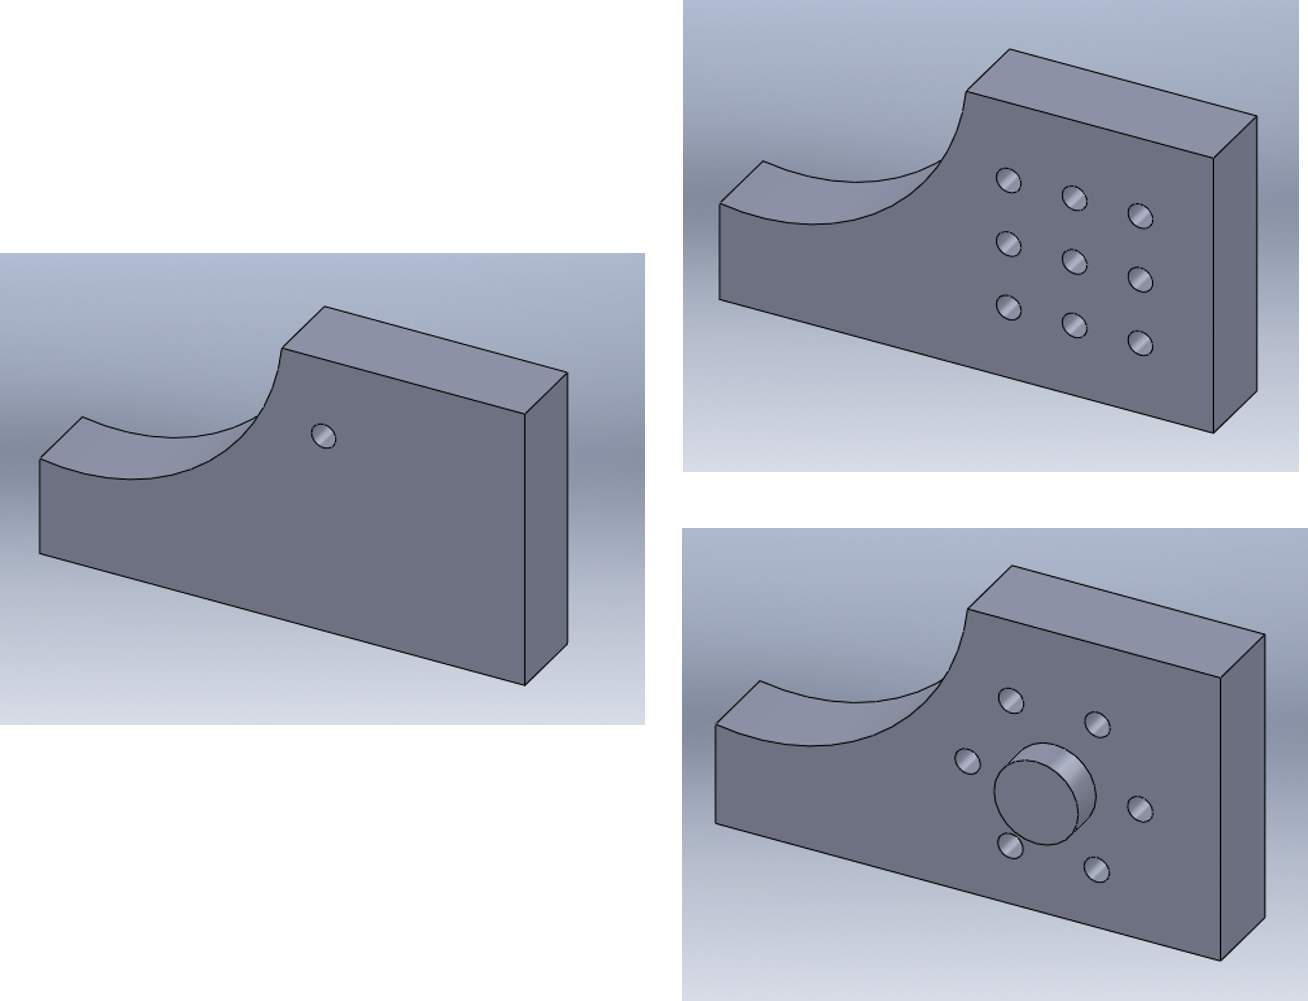
\includegraphics[width=0.9\linewidth,keepaspectratio]{geomod38}
			\end{center}
\end{frame}

%%%%%%%%%%%%%%%%%%%%%%%%%%%%%%%%%%%%%%%%%%%%%%%%%%%%%%%%%%%%%%%%%%%%%%%%%%%%%%%%%%
\begin{frame}[fragile]\frametitle{Summay}

\begin{itemize}
\item Most CAD systems use solid, parametric, feature-based modeling
\item Parts are modeled by adding features to a base feature
\item Features can be easily added, deleted and modified
\end{itemize}
\end{frame}
